\documentclass[11pt,usenames,dvipsnames,
hyperref={pdfencoding=auto,psdextra}]{beamer}
\def\showTODOs{}


\usepackage{gensymb}

\newcommand*{\listsofb}[1]{\mathcal{L} (#1)}
\newcommand*{\listsof}{\mathcal{L}~}

\newcommand{\None}{\emptyset}
\newcommand{\Some}[1]{\degree\kern-0.5ex#1}
\newcommand{\lnil}{\ensuremath{[]}}

\newcommand*{\match}{\textbf{match}~}
\newcommand*{\withl}{\textbf{[}~}
\newcommand*{\withr}{~\textbf{]}}
\newcommand*{\withm}{\quad\textbf{|}\quad}
\newcommand*{\llet}{\textbf{let}~}
\newcommand*{\lin}{\textbf{in}~}
\newcommand{\ITE}[3]{\textbf{if}~{#1}~\textbf{then}~{#2}~\textbf{else}~{#3}}

\newcommand{\Type}{\mathbb{T}}
\newcommand{\Prop}{\mathbb{P}}
\newcommand{\bool}{\mathbb{B}}
\newcommand{\btrue}{\mathsf{T}}
\newcommand{\bfalse}{\mathsf{F}}
\newcommand{\andb}{\&\&}
\newcommand{\orb}{||}
\newcommand{\notb}{!}
\newcommand{\nat}{\mathbb{N}}
\newcommand{\natS}{1 + }
\newcommand{\length}[1]{|#1|}

\newcommand{\con}{\mathop{{+}\!\!\!{+}}}
\newcommand{\rev}{\mathsf{rev}}
\newcommand{\opt}[1]{\mathcal{O}{#1}}

\newcommand{\eqb}[2]{#1\overset{?}{=}#2}

\usepackage[english]{babel}
\usepackage{lipsum}
\usepackage{pifont}
\usepackage{booktabs}
\usepackage{multirow}
\usepackage[absolute,overlay]{textpos}
\usepackage{proof}
\usepackage{amsmath}
%\usepackage[utf8]{inputenc}
\usepackage{listings}
\usepackage{tikz}
\usetikzlibrary{automata,trees,calc,arrows.meta,positioning,decorations.pathreplacing,bending,shapes.geometric, intersections, hobby}
\usetheme{Berlin}
\usepackage{cite}
\usepackage{cancel}
\usepackage{xsavebox}
\usepackage[normalem]{ulem}
\usepackage{array}
%\usepackage{wasysym}
\usepackage{stmaryrd}
\usepackage{pgfplots}
\usepackage{ifthen}


\pgfplotsset{compat=1.16}

%some nicer colour scheme
\definecolor{craneorange}{RGB}{237, 142, 26}
\definecolor{craneblue}{RGB}{0,0,0}

\setbeamercolor{structure}{fg=craneblue}

\setbeamercolor{palette primary}{fg=craneblue,bg=craneorange!70}
\setbeamercolor{palette secondary}{fg=craneblue,bg=craneorange!80}
\setbeamercolor{palette tertiary}{fg=craneblue,bg=craneorange!90}
\setbeamercolor{palette quaternary}{fg=craneblue,bg=craneorange}

\setbeamercolor{titlelike}{parent=palette quaternary}

\setbeamercolor{block title}{fg=craneblue,bg=craneorange}
\setbeamercolor{block title alerted}{use=alerted text,fg=craneblue,bg=alerted text.fg!75!bg}
\setbeamercolor{block title example}{use=example text,fg=craneblue,bg=example text.fg!75!bg}

\setbeamercolor{block body}{parent=normal text,use=block title,bg=block title.bg!15!bg}
\setbeamercolor{block body alerted}{parent=normal text,use=block title alerted,bg=block title alerted.bg!15!bg}
\setbeamercolor{block body example}{parent=normal text,use=block title example,bg=block title example.bg!15!bg}

\setbeamercolor{sidebar}{bg=craneorange!70}

\setbeamercolor{palette sidebar primary}{fg=craneblue}
\setbeamercolor{palette sidebar secondary}{fg=craneblue!75}
\setbeamercolor{palette sidebar tertiary}{fg=craneblue!75}
\setbeamercolor{palette sidebar quaternary}{fg=craneblue}

\setbeamercolor*{separation line}{}
\setbeamercolor*{fine separation line}{}

\setbeamercolor{frametitle}{bg=white}

%no frame numbering when using framebreaks
\setbeamertemplate{frametitle continuation}{}

%no total frame number
\setbeamertemplate{footline}{% 
  \hfill% 
  \usebeamercolor[fg]{page number in head/foot}% 
  \usebeamerfont{page number in head/foot}% 
  \insertframenumber%
  %\,/\,\inserttotalframenumber
  \kern1em\vskip2pt% 
}

%no subsection line
\setbeamertemplate{headline}
{%
  \begin{beamercolorbox}[colsep=1.5pt]{upper separation line head}
  \end{beamercolorbox}
  \begin{beamercolorbox}{section in head/foot}
    \vskip0pt\insertnavigation{\paperwidth}\vskip3pt
  \end{beamercolorbox}%
  \begin{beamercolorbox}[colsep=1.5pt]{lower separation line head}
  \end{beamercolorbox}
}

%highlight colours to be used throughout the presentation
\newcommand{\highlight}[1]{\color{blue}#1\color{black}}
\newcommand{\colorHOne}{\color{red}}
\newcommand{\colorHThree}{\color{violet}}
\newcommand{\colorHTwo}{\color{blue}}
\newcommand{\colorHFour}{\color{green}}

\newcommand{\colorTikzA}{red}
\newcommand{\colorTikzB}{cyan}
\newcommand{\colorTikzC}{blue}
\newcommand{\colorTikzD}{green}
\newcommand{\colorTikzE}{violet}

%don't count the title page
\let\otp\titlepage
\renewcommand{\titlepage}{\otp\addtocounter{framenumber}{-1}}

%a hide on=... option for tikz elements, where the usual ranges allowed by \only are allowed for ...
\tikzset{hide on/.code={\only<#1>{\pgfkeysalso{white}}}}

%don't want those nasty navigation symbols
\beamertemplatenavigationsymbolsempty


\newenvironment{tightcenter}{%
  \setlength\topsep{0pt}
  \setlength\parskip{0pt}
  \begin{center}
    }{%
  \end{center}
}

%table column types for fixed width
\newcolumntype{L}[1]{>{\raggedright\let\newline\\\arraybackslash\hspace{0pt}}m{#1}}
\newcolumntype{C}[1]{>{\centering\let\newline\\\arraybackslash\hspace{0pt}}m{#1}}
\newcolumntype{R}[1]{>{\raggedleft\let\newline\\\arraybackslash\hspace{0pt}}m{#1}}

\newcommand{\TODO}[1]{\ifthenelse{\isundefined{\showTODOs}}{}{\colorbox{red}{\LARGE TODO}:#1}}


%math stuff
\newcommand*{\Eq}{\text{Eq}}
\newcommand*{\N}{\mathbb{N}}
\newcommand*{\R}{\mathbb{R}}
\newcommand*{\Reach}{\text{Reach}}
\newcommand*{\norm}[1]{\left\lVert#1\right\rVert}
\newcommand*{\diff}{\text{d}}
\newcount\colveccount
\newcommand*\colvec[1]{
  \global\colveccount#1
  \begin{pmatrix}
    \colvecnext
  }
  \def\colvecnext#1{
    #1
    \global\advance\colveccount-1
    \ifnum\colveccount>0
      \\
      \expandafter\colvecnext
    \else
    \end{pmatrix}
  \fi
}


%prevent backup slides from appearing in the header
\makeatletter
\let\beamer@writeslidentry@miniframeson=\beamer@writeslidentry%
\def\beamer@writeslidentry@miniframesoff{%
  \expandafter\beamer@ifempty\expandafter{\beamer@framestartpage}{}% does not happen normally
  {%else
    % removed \addtocontents commands
    \clearpage\beamer@notesactions%
  }
}
\newcommand*{\miniframeson}{\let\beamer@writeslidentry=\beamer@writeslidentry@miniframeson}
\newcommand*{\miniframesoff}{\let\beamer@writeslidentry=\beamer@writeslidentry@miniframesoff}
\makeatother


%footnote without marker, for images
\newcommand\blfootnote[1]{%
  \begingroup
  \renewcommand\thefootnote{}\footnote{#1}%
  \addtocounter{footnote}{-1}%
  \endgroup
}

\newcommand{\bnfmid}{~\mid~}

\newcommand*{\PR}{\textbf{PR}}
\newcommand*{\sat}{\textbf{SAT}}
\newcommand*{\gennp}{\textbf{GenNP}}
\newcommand{\fsat}{\textbf{FSAT}}
\newcommand{\NP}{\textsf{NP}}

\newcolumntype{C}{>{$}c<{$}}
\newcommand{\rewwin}[2]{
  \begin{tabular}{C|C|C}
    #1 \\ 
    \midrule #2
  \end{tabular}
}

\newcommand{\trewwin}[6]{
  \begin{tikzpicture}
    \draw (0, 0) -- (2.25, 0);
    \draw (0.75, -0.75) -- (0.75, 0.75);
    \draw (1.5, -0.75) -- (1.5, 0.75);
    \node at (0.375, 0.375) {\ensuremath{#1}};
    \node at (0.375, -0.375) {\ensuremath{#4}};
    \node at (1.125, 0.375) {\ensuremath{#2}};
    \node at (1.125, -0.375) {\ensuremath{#5}};
    \node at (1.875, 0.375) {\ensuremath{#3}};
    \node at (1.875, -0.375) {\ensuremath{#6}};
  \end{tikzpicture}
}

\newcommand{\polneg}[1]{\overleftarrow{#1}}
\newcommand{\polpos}[1]{\overrightarrow{#1}}
\newcommand{\polneut}[1]{\overline{#1}}

\newcommand{\reprt}[1]{\ensuremath{\sim_t^{#1}}}
\newcommand{\reprtt}[2]{\ensuremath{\sim_t^{(#1, #2)}}}
\newcommand{\reprc}{\ensuremath{\sim_c}}



\newcommand{\strent}{\rightsquigarrow}
\newcommand{\constrent}{\overset{!}{\rightsquigarrow}}
\newcommand{\Rfinal}{R_{\text{final}}}

\newcommand{\blank}{\textbf{\textvisiblespace}}


\title{Towards a Formalisation of Cook's Theorem in Coq}

\institute{Saarland University}
\date{10 January 2020}
\author{Lennard Gäher\\[1mm] {\small{Advisor: Fabian Kunze}}}

\begin{document}
\begin{frame}[plain]
  \titlepage
\end{frame}

\section{Introduction}

\begin{frame}{Cook's Theorem (1971)}

  \begin{block}{\vspace*{-3ex}}
    The satisfiability problem on CNFs \sat{} is NP-hard.
  \end{block}
  \begin{center}
    \color{gray}
    Given a Boolean formula in conjunctive normal form, does there exist a satisfying assignment?
  \end{center}
\end{frame}

\begin{frame}{Generic NP-hard Problem on Turing Machines}
  \begin{block}{GenNP}
    \begin{overlayarea}{\textwidth}{0.25\textwidth}
      \only<1>{
        \begin{align*}
          \textbf{GenNP}~(M, \mathit{input}, t) := &M \text{ is a nondet.\ 1-tape TM} \\
          \land & M \text{ accepts on } \mathit{input} \text{ in } \le t \text{ steps}
        \end{align*}
      }
      \only<2->{
        \begin{align*}
          \textbf{GenNP}~(M, k, t) := &M \text{ is a det.\ 1-tape TM} \\
          \land & \exists~\mathit{input}, \length{input} \le k \\
                &\quad \land M \text{ accepts on } \mathit{input} \text{ in } \le t \text{ steps}
        \end{align*}
      }
    \end{overlayarea}
  \end{block}

  \onslide<3->
  \[ 
    (M, k, t) \in \gennp{} \leftrightarrow f(M, k, t) \in \sat{}
  \]
\end{frame}

\begin{frame}{Challenges}
  \begin{itemize}
    \item \sat{} formula has a fixed size, but: 
      \begin{itemize} 
        \item TM may have different space usage depending on input
        \item TM may take a different number of steps until it halts
      \end{itemize}
    \item nondeterministically ``guess'' input
    \item encode arbitrary alphabet using Boolean variables
  \end{itemize}
  %tackle these problems with a sequence of intermediate languages
\end{frame}

\section{Parallel Rewriting}
\begin{frame}[t]{String-based Configurations}
  \begin{overlayarea}{\textwidth}{0.08\textwidth}
    \color{gray}
    \begin{minipage}{0.48\textwidth}
      $\Sigma = \{a, b, c\}$
    \end{minipage}
    \begin{minipage}{0.48\textwidth}
      \raggedleft
      $\delta(q_1, a) = (q_2, \Some{b}, \textsf{L})$
    \end{minipage}
  \end{overlayarea}
  \begin{overlayarea}{\textwidth}{0.3\textwidth}
    \begin{center}
      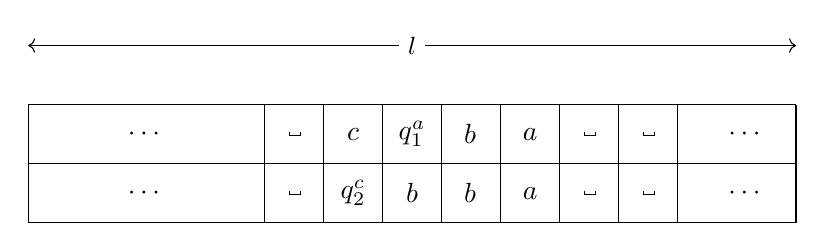
\begin{tikzpicture}
        \draw (0, 0.75) -- (9.75, 0.75);
        \draw (0, 0) -- (9.75, 0);
        \draw (0, 0) -- (0, 0.75);
        \draw (9.75, 0) -- (9.75, 0.75);

        \draw (4.5, 0) -- (4.5, 0.75);
        \draw (5.25, 0) -- (5.25, 0.75);
        \draw (3.75, 0) -- (3.75, 0.75);
        \draw (3, 0) -- (3, 0.75);
        \draw (6, 0) -- (6, 0.75);
        \draw (6.75, 0) -- (6.75, 0.75);
        \draw (7.5, 0) -- (7.5, 0.75);
        \draw (8.25, 0) -- (8.25, 0.75);

        %\node at (5.6125, 1) {\small$1$};
        %\node at (6.375, 1) {\small$2$};
        %\node at (7.125, 1) {\small$3$};
        %\node at (4.875, 1) {\small$0$};
        %\node at (4.125, 1) {\small$-1$};
        %\node at (3.375, 1) {\small$-2$};

        \node at (1.5, 0.375) {$\cdots$};
        \node at (9.125, 0.375) {$\cdots$};
        \node at (5.6125, 0.375) {$b$};
        \node at (6.375, 0.375) {$a$};
        \node at (7.125, 0.375) {\blank};
        \node at (7.875, 0.375) {\blank};
        \node at (4.875, 0.375) {$q_1^a$};
        \node at (4.125, 0.375) {$c$};
        \node at (3.375, 0.375) {\blank};

        \path[<->] (0, 1.5) edge node[fill=white, anchor=center, pos= 0.5] {\small $l$} (9.75, 1.5);
        %\path[<->] (0, -0.5) edge node[fill=white, anchor=center, pos =0.5] {\small $z$} (5, -0.5);

        \onslide<2-> {
          \draw (0, -0.75) -- (9.75, -0.75);
          \draw (0, -0.75) -- (0, 0);
          \draw (9.75, -0.75) -- (9.75, 0);

          \draw (4.5, 0) -- (4.5, -0.75);
          \draw (5.25, 0) -- (5.25, -0.75);
          \draw (3.75, 0) -- (3.75, -0.75);
          \draw (3, 0) -- (3, -0.75);
          \draw (6, 0) -- (6, -0.75);
          \draw (6.75, 0) -- (6.75, -0.75);
          \draw (7.5, 0) -- (7.5, -0.75);
          \draw (8.25, 0) -- (8.25, -0.75);

          \node at (1.5, -0.375) {$\cdots$};
          \node at (9.125, -0.375) {$\cdots$};
          \node at (5.6125, -0.375) {$b$};
          \node at (6.375, -0.375) {$a$};
          \node at (7.125, -0.375) {\blank};
          \node at (7.875, -0.375) {\blank};
          \node at (4.875, -0.375) {$b$};
          \node at (4.125, -0.375) {$q_2^c$};
          \node at (3.375, -0.375) {\blank};
        }
      \end{tikzpicture}
    \end{center}
  \end{overlayarea}

  \onslide<4-> {
    {\colorHOne{} Non-unique representation: }
    \begin{center}
      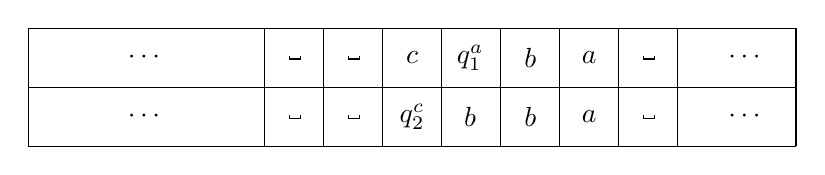
\begin{tikzpicture}
        \draw (0, 0.75) -- (9.75, 0.75);
        \draw (0, 0) -- (9.75, 0);
        \draw (0, 0) -- (0, 0.75);
        \draw (9.75, 0) -- (9.75, 0.75);

        \draw (4.5, 0) -- (4.5, 0.75);
        \draw (5.25, 0) -- (5.25, 0.75);
        \draw (3.75, 0) -- (3.75, 0.75);
        \draw (3, 0) -- (3, 0.75);
        \draw (6, 0) -- (6, 0.75);
        \draw (6.75, 0) -- (6.75, 0.75);
        \draw (7.5, 0) -- (7.5, 0.75);
        \draw (8.25, 0) -- (8.25, 0.75);

        \node at (1.5, 0.375) {$\cdots$};
        \node at (9.125, 0.375) {$\cdots$};
        \node at (5.6125, 0.375) {$q_1^a$};
        \node at (6.375, 0.375) {$b$};
        \node at (7.125, 0.375) {$a$};
        \node at (7.875, 0.375) {\blank};
        \node at (4.875, 0.375) {$c$};
        \node at (4.125, 0.375) {\blank};
        \node at (3.375, 0.375) {\blank};

        \draw (0, -0.75) -- (9.75, -0.75);
        \draw (0, -0.75) -- (0, 0);
        \draw (9.75, -0.75) -- (9.75, 0);

        \draw (4.5, 0) -- (4.5, -0.75);
        \draw (5.25, 0) -- (5.25, -0.75);
        \draw (3.75, 0) -- (3.75, -0.75);
        \draw (3, 0) -- (3, -0.75);
        \draw (6, 0) -- (6, -0.75);
        \draw (6.75, 0) -- (6.75, -0.75);
        \draw (7.5, 0) -- (7.5, -0.75);
        \draw (8.25, 0) -- (8.25, -0.75);

        \node at (1.5, -0.375) {$\cdots$};
        \node at (9.125, -0.375) {$\cdots$};
        \node at (5.6125, -0.375) {$b$};
        \node at (6.375, -0.375) {$b$};
        \node at (7.125, -0.375) {$a$};
        \node at (7.875, -0.375) {\blank};
        \node at (4.875, -0.375) {$q_2^c$};
        \node at (4.125, -0.375) {\blank};
        \node at (3.375, -0.375) {\blank};
      \end{tikzpicture}
    \end{center}
  }
\end{frame}

\begin{frame}[t]{Fixed State Position}
  \begin{overlayarea}{\textwidth}{0.08\textwidth}
    \color{gray}
    \begin{minipage}{0.48\textwidth}
      $\Sigma = \{a, b, c\}$
    \end{minipage}
    \begin{minipage}{0.48\textwidth}
      \onslide<2->{
        \raggedleft
        $\delta(q_1, a) = (q_2, \Some{b}, \textsf{L})$
      }
    \end{minipage}
  \end{overlayarea}
  \begin{overlayarea}{\textwidth}{0.3\textwidth}
    \begin{center}
      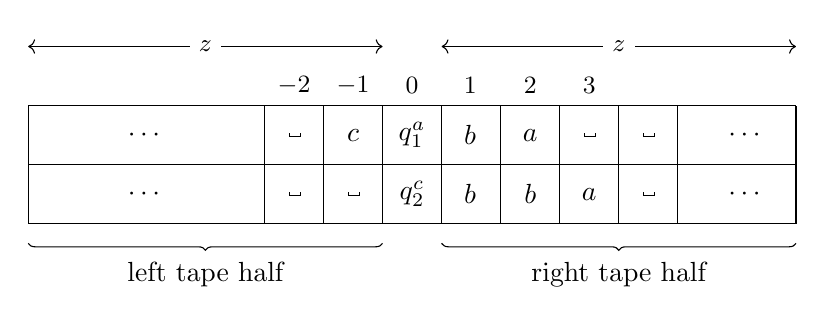
\begin{tikzpicture}
        \draw (0, 0.75) -- (9.75, 0.75);
        \draw (0, 0) -- (9.75, 0);
        \draw (0, 0) -- (0, 0.75);
        \draw (9.75, 0) -- (9.75, 0.75);

        \draw (4.5, 0) -- (4.5, 0.75);
        \draw (5.25, 0) -- (5.25, 0.75);
        \draw (3.75, 0) -- (3.75, 0.75);
        \draw (3, 0) -- (3, 0.75);
        \draw (6, 0) -- (6, 0.75);
        \draw (6.75, 0) -- (6.75, 0.75);
        \draw (7.5, 0) -- (7.5, 0.75);
        \draw (8.25, 0) -- (8.25, 0.75);

        \node at (5.6125, 1) {\small$1$};
        \node at (6.375, 1) {\small$2$};
        \node at (7.125, 1) {\small$3$};
        \node at (4.875, 1) {\small$0$};
        \node at (4.125, 1) {\small$-1$};
        \node at (3.375, 1) {\small$-2$};

        \node at (1.5, 0.375) {$\cdots$};
        \node at (9.125, 0.375) {$\cdots$};
        \node at (5.6125, 0.375) {$b$};
        \node at (6.375, 0.375) {$a$};
        \node at (7.125, 0.375) {\blank};
        \node at (7.875, 0.375) {\blank};
        \node at (4.875, 0.375) {$q_1^a$};
        \node at (4.125, 0.375) {$c$};
        \node at (3.375, 0.375) {\blank};

        \path[<->] (0, 1.5) edge node[fill=white, anchor=center, pos= 0.5] {\small $z$} (4.5, 1.5);
        \node[color=white] at (4.75, 1.5) {l};
        \path[<->] (5.25, 1.5) edge node[fill=white, anchor=center, pos =0.5] {\small $z$} (9.75, 1.5);

        \onslide<2-> {
          \draw (0, -0.75) -- (9.75, -0.75);
          \draw (0, -0.75) -- (0, 0);
          \draw (9.75, -0.75) -- (9.75, 0);

          \draw (4.5, 0) -- (4.5, -0.75);
          \draw (5.25, 0) -- (5.25, -0.75);
          \draw (3.75, 0) -- (3.75, -0.75);
          \draw (3, 0) -- (3, -0.75);
          \draw (6, 0) -- (6, -0.75);
          \draw (6.75, 0) -- (6.75, -0.75);
          \draw (7.5, 0) -- (7.5, -0.75);
          \draw (8.25, 0) -- (8.25, -0.75);

          \node at (1.5, -0.375) {$\cdots$};
          \node at (9.125, -0.375) {$\cdots$};
          \node at (5.6125, -0.375) {$b$};
          \node at (6.375, -0.375) {$b$};
          \node at (7.125, -0.375) {$a$};
          \node at (7.875, -0.375) {\blank};
          \node at (4.875, -0.375) {$q_2^c$};
          \node at (4.125, -0.375) {\blank};
          \node at (3.375, -0.375) {\blank};
        }

        \draw[decorate, decoration={brace, mirror}] (0, -1) -- (4.5, -1) node[midway, yshift=-0.4cm] {left tape half};
        \draw[decorate, decoration={brace, mirror}] (5.25, -1) -- (9.75, -1) node[midway, yshift=-0.4cm] {right tape half};
      \end{tikzpicture}
    \end{center}
  \end{overlayarea}
\end{frame}

\begin{frame}[t]{Rewrite Windows: Force Valid Configuration Changes}
  \begin{overlayarea}{\textwidth}{0.08\textwidth}
    \color{gray}
    \begin{minipage}{0.48\textwidth}
      $\Sigma = \{a, b, c\}$
    \end{minipage}
    \begin{minipage}{0.48\textwidth}
      \onslide<1->{
      \raggedleft
      $\delta(q_1, a) = (q_2, \Some{b}, \textsf{L})$
    }
    \end{minipage}
  \end{overlayarea}
  \begin{overlayarea}{\textwidth}{0.3\textwidth}
    \begin{center}
      \begin{tikzpicture}
        \draw (0, 0.75) -- (9.75, 0.75);
        \draw (0, 0) -- (9.75, 0);
        \draw (0, 0) -- (0, 0.75);
        \draw (9.75, 0) -- (9.75, 0.75);

        \draw (4.5, 0) -- (4.5, 0.75);
        \draw (5.25, 0) -- (5.25, 0.75);
        \draw (3.75, 0) -- (3.75, 0.75);
        \draw (3, 0) -- (3, 0.75);
        \draw (6, 0) -- (6, 0.75);
        \draw (6.75, 0) -- (6.75, 0.75);
        \draw (7.5, 0) -- (7.5, 0.75);
        \draw (8.25, 0) -- (8.25, 0.75);

        \node at (5.6125, 1) {\small$1$};
        \node at (6.375, 1) {\small$2$};
        \node at (7.125, 1) {\small$3$};
        \node at (4.875, 1) {\small$0$};
        \node at (4.125, 1) {\small$-1$};
        \node at (3.375, 1) {\small$-2$};

        \node at (1.5, 0.375) {$\cdots$};
        \node at (9.125, 0.375) {$\cdots$};
        \node at (5.6125, 0.375) {\only<2-4>{\colorHTwo}$b$};
        \node at (6.375, 0.375) {\only<3-4>{\colorHTwo}$a$};
        \node at (7.125, 0.375) {\only<4>{\colorHTwo}\blank};
        \node at (7.875, 0.375) {\blank};
        \node at (4.875, 0.375) {\only<2-3>{\colorHTwo}$q_1^a$};
        \node at (4.125, 0.375) {\only<2>{\colorHTwo}$c$};
        \node at (3.375, 0.375) {\blank};

        \path[<->] (0, 1.5) edge node[fill=white, anchor=center, pos= 0.5] {\small $z$} (4.5, 1.5);
        \node[color=white] at (4.75, 1.5) {l};
        \path[<->] (5.25, 1.5) edge node[fill=white, anchor=center, pos =0.5] {\small $z$} (9.75, 1.5);

          \draw (0, -0.75) -- (9.75, -0.75);
          \draw (0, -0.75) -- (0, 0);
          \draw (9.75, -0.75) -- (9.75, 0);

          \draw (4.5, 0) -- (4.5, -0.75);
          \draw (5.25, 0) -- (5.25, -0.75);
          \draw (3.75, 0) -- (3.75, -0.75);
          \draw (3, 0) -- (3, -0.75);
          \draw (6, 0) -- (6, -0.75);
          \draw (6.75, 0) -- (6.75, -0.75);
          \draw (7.5, 0) -- (7.5, -0.75);
          \draw (8.25, 0) -- (8.25, -0.75);

          \node at (1.5, -0.375) {$\cdots$};
          \node at (9.125, -0.375) {$\cdots$};
          \node at (5.6125, -0.375) {\only<2-4>{\colorHTwo}$b$};
          \node at (6.375, -0.375) {\only<3-4>{\colorHTwo}$b$};
          \node at (7.125, -0.375) {\only<4>{\colorHTwo}$a$};
          \node at (7.875, -0.375) {\blank};
          \node at (4.875, -0.375) {\only<2-3>{\colorHTwo}$q_2^c$};
          \node at (4.125, -0.375) {\only<2>{\colorHTwo}\blank};
          \node at (3.375, -0.375) {\blank};

        \only<2>{
          \draw[color=\colorTikzC] (4.5, -0.75) -- (4.5, 0.75);
          \draw[color=\colorTikzC] (5.25, -0.75) -- (5.25, 0.75);
          \draw[color=\colorTikzC] (3.75, 0) -- (6, 0);
        }
        \only<3>{
          \draw[color=\colorTikzC] (5.25, -0.75) -- (5.25, 0.75);
          \draw[color=\colorTikzC] (6, -0.75) -- (6, 0.75);
          \draw[color=\colorTikzC] (4.5, 0) -- (6.75, 0);

        }
      \end{tikzpicture}
    \end{center}
  \end{overlayarea}

  \onslide<2->
  \begin{center}
    %\rewwin{\blank & \blank & c}{\blank & \blank & \blank}
    %\rewwin{\blank & c & q_1^a}{\blank & \blank & q_2^c}
    {
      \only<2>{\colorHTwo}
      \trewwin{c}{q_1^a}{b}{\blank}{q_2^c}{b}
    }
    \onslide<3->
    {
      \only<3>{\colorHTwo}
      \trewwin{q_1^a}{b}{a}{q_2^c}{b}{b}
    }
    \onslide<4->
    {
      \only<4>{\colorHTwo}
      \trewwin{b}{a}{\blank}{b}{b}{a}
    }
  \end{center}


\end{frame}

\begin{frame}[t]{Tape Shifts}
  Add one symbol to the right half of the tape:
  \begin{overlayarea}{\textwidth}{0.15\textwidth}
    \vspace{-0.5ex}
    \begin{minipage}{0.58\textwidth}
      \begin{center}
        \begin{tikzpicture}
          \draw (5.25, 0.75) -- (9.75, 0.75);
          \draw (5.25, 0) -- (9.75, 0);
          \draw (5.25, 0) -- (5.25, 0.75);
          \draw (9.75, 0) -- (9.75, 0.75);

          \draw (5.25, 0) -- (5.25, 0.75);
          \draw (6, 0) -- (6, 0.75);
          \draw (6.75, 0) -- (6.75, 0.75);
          \draw (7.5, 0) -- (7.5, 0.75);
          \draw (8.25, 0) -- (8.25, 0.75);

          \node at (9.125, 0.375) {$\cdots$};
          \node at (7.125, 0.375) {\blank};
          \node at (7.875, 0.375) {\blank};
          \only<1>{
            \node at (5.6125, 0.375) {$b$};
            \node at (6.375, 0.375) {$a$};
          }
          \only<2->{ 
            \node at (5.6125, 0.375) {$\sigma_1$};
            \node at (6.375, 0.375) {$\sigma_2$};
          }


          \draw (5.25, -0.75) -- (9.75, -0.75);
          \draw (5.25, -0.75) -- (5.25, 0);
          \draw (9.75, -0.75) -- (9.75, 0);

          \draw (5.25, 0) -- (5.25, -0.75);
          \draw (6, 0) -- (6, -0.75);
          \draw (6.75, 0) -- (6.75, -0.75);
          \draw (7.5, 0) -- (7.5, -0.75);
          \draw (8.25, 0) -- (8.25, -0.75);

          \node at (9.125, -0.375) {$\cdots$};
          \node at (7.875, -0.375) {\blank};
          \only<1>{
            \node at (5.6125, -0.375) {$b$};
            \node at (6.375, -0.375) {$b$};
            \node at (7.125, -0.375) {$a$};
          }
          \only<2->{
            \node at (5.6125, -0.375) {$\sigma_3$};
            \node at (6.375, -0.375) {$\sigma_1$};
            \node at (7.125, -0.375) {$\sigma_2$};
          }
        \end{tikzpicture}
      \end{center}
    \end{minipage}
    \begin{minipage}{0.38\textwidth}
      \trewwin{\only<1>{b}\only<2->{\sigma_1}}{\only<1>{a}\only<2->{\sigma_2}}{\blank}{\only<1>{b}\only<2->{\sigma_3}}{\only<1>{b}\only<2->{\sigma_1}}{\only<1>{a}\only<2->{\sigma_2}}
    \end{minipage}
  \end{overlayarea}

  \vspace{2ex}

  \onslide<3->
  Leave the tape unchanged:

  \begin{overlayarea}{\textwidth}{0.15\textwidth}
    \vspace{-0.5ex}
    \begin{minipage}{0.58\textwidth}
      \begin{center}
        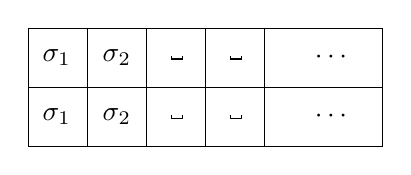
\begin{tikzpicture}
          \draw (5.25, 0.75) -- (9.75, 0.75);
          \draw (5.25, 0) -- (9.75, 0);
          \draw (5.25, 0) -- (5.25, 0.75);
          \draw (9.75, 0) -- (9.75, 0.75);

          \draw (5.25, 0) -- (5.25, 0.75);
          \draw (6, 0) -- (6, 0.75);
          \draw (6.75, 0) -- (6.75, 0.75);
          \draw (7.5, 0) -- (7.5, 0.75);
          \draw (8.25, 0) -- (8.25, 0.75);

          \node at (9.125, 0.375) {$\cdots$};
          \node at (7.125, 0.375) {\blank};
          \node at (7.875, 0.375) {\blank};
          \node at (5.6125, 0.375) {$\sigma_1$};
          \node at (6.375, 0.375) {$\sigma_2$};


          \draw (5.25, -0.75) -- (9.75, -0.75);
          \draw (5.25, -0.75) -- (5.25, 0);
          \draw (9.75, -0.75) -- (9.75, 0);

          \draw (5.25, 0) -- (5.25, -0.75);
          \draw (6, 0) -- (6, -0.75);
          \draw (6.75, 0) -- (6.75, -0.75);
          \draw (7.5, 0) -- (7.5, -0.75);
          \draw (8.25, 0) -- (8.25, -0.75);

          \node at (9.125, -0.375) {$\cdots$};
          \node at (7.125, -0.375) {\blank};
          \node at (7.875, -0.375) {\blank};
          \node at (5.6125, -0.375) {$\sigma_1$};
          \node at (6.375, -0.375) {$\sigma_2$};
        \end{tikzpicture}
      \end{center}
    \end{minipage}
    \begin{minipage}{0.38\textwidth}
      \only<5>{\colorHOne}
      \trewwin{\sigma_1}{\sigma_2}{\blank}{\sigma_1}{\sigma_2}{\blank}
    \end{minipage}
  \end{overlayarea}

  \vspace{2ex}
  \onslide<4->
  \begin{center}

    \begin{tikzpicture}
      \draw (0, 0.75) -- (9.75, 0.75);
      \draw (0, 0) -- (9.75, 0);
      \draw (0, 0) -- (0, 0.75);
      \draw (9.75, 0) -- (9.75, 0.75);

      \draw (4.5, 0) -- (4.5, 0.75);
      \draw (5.25, 0) -- (5.25, 0.75);
      \draw (3.75, 0) -- (3.75, 0.75);
      \draw (3, 0) -- (3, 0.75);
      \draw (6, 0) -- (6, 0.75);
      \draw (6.75, 0) -- (6.75, 0.75);
      \draw (7.5, 0) -- (7.5, 0.75);
      \draw (8.25, 0) -- (8.25, 0.75);

      %\node at (5.6125, 1) {\small$1$};
      %\node at (6.375, 1) {\small$2$};
      %\node at (7.125, 1) {\small$3$};
      %\node at (4.875, 1) {\small$0$};
      %\node at (4.125, 1) {\small$-1$};
      %\node at (3.375, 1) {\small$-2$};

      \node at (1.5, 0.375) {$\cdots$};
      \node at (9.125, 0.375) {$\cdots$};
      \node at (5.6125, 0.375) {\only<5->{\colorHOne}$b$};
      \node at (6.375, 0.375) {\only<5->{\colorHOne}$a$};
      \node at (7.125, 0.375) {\only<5->{\colorHOne}\blank};
      \node at (7.875, 0.375) {\blank};
      \node at (4.875, 0.375) {$q_1^a$};
      \node at (4.125, 0.375) {$c$};
      \node at (3.375, 0.375) {\blank};

      %\path[<->] (0, 1.5) edge node[fill=white, anchor=center, pos= 0.5] {\small $z$} (4.5, 1.5);
      %\node[color=white] at (4.75, 1.5) {l};
      %\path[<->] (5.25, 1.5) edge node[fill=white, anchor=center, pos =0.5] {\small $z$} (9.75, 1.5);

      \draw (0, -0.75) -- (9.75, -0.75);
      \draw (0, -0.75) -- (0, 0);
      \draw (9.75, -0.75) -- (9.75, 0);

      \draw (4.5, 0) -- (4.5, -0.75);
      \draw (5.25, 0) -- (5.25, -0.75);
      \draw (3.75, 0) -- (3.75, -0.75);
      \draw (3, 0) -- (3, -0.75);
      \draw (6, 0) -- (6, -0.75);
      \draw (6.75, 0) -- (6.75, -0.75);
      \draw (7.5, 0) -- (7.5, -0.75);
      \draw (8.25, 0) -- (8.25, -0.75);

      \node at (1.5, -0.375) {$\cdots$};
      \node at (9.125, -0.375) {$\cdots$};
      \node at (5.6125, -0.375) {\only<5->{\colorHOne{}} $b$};
      \node at (6.375, -0.375) {\only<4>{b}\only<5->{\colorHOne{}$a$}};
      \node at (7.125, -0.375) {\only<4>{a}\only<5->{\colorHOne{}\blank}};
      \node at (7.875, -0.375) {\blank};
      \node at (4.875, -0.375) {$q_2^c$};
      \node at (4.125, -0.375) {\blank};
      \node at (3.375, -0.375) {\blank};
    \end{tikzpicture}
  \end{center}
\end{frame}

\begin{frame}{Polarities}
  Add one symbol to the right half of the tape:
  \begin{overlayarea}{\textwidth}{0.15\textwidth}
    \vspace{-0.5ex}
    \begin{minipage}{0.58\textwidth}
      \begin{center}
        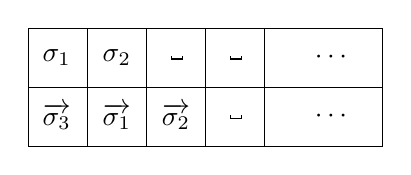
\begin{tikzpicture}
          \draw (5.25, 0.75) -- (9.75, 0.75);
          \draw (5.25, 0) -- (9.75, 0);
          \draw (5.25, 0) -- (5.25, 0.75);
          \draw (9.75, 0) -- (9.75, 0.75);

          \draw (5.25, 0) -- (5.25, 0.75);
          \draw (6, 0) -- (6, 0.75);
          \draw (6.75, 0) -- (6.75, 0.75);
          \draw (7.5, 0) -- (7.5, 0.75);
          \draw (8.25, 0) -- (8.25, 0.75);

          \node at (9.125, 0.375) {$\cdots$};
          \node at (7.125, 0.375) {\blank};
          \node at (7.875, 0.375) {\blank};

          \node at (5.6125, 0.375) {$\sigma_1$};
          \node at (6.375, 0.375) {$\sigma_2$};


          \draw (5.25, -0.75) -- (9.75, -0.75);
          \draw (5.25, -0.75) -- (5.25, 0);
          \draw (9.75, -0.75) -- (9.75, 0);

          \draw (5.25, 0) -- (5.25, -0.75);
          \draw (6, 0) -- (6, -0.75);
          \draw (6.75, 0) -- (6.75, -0.75);
          \draw (7.5, 0) -- (7.5, -0.75);
          \draw (8.25, 0) -- (8.25, -0.75);

          \node at (9.125, -0.375) {$\cdots$};
          \node at (7.875, -0.375) {\blank};
          \node at (5.6125, -0.375) {$\polpos{\sigma_3}$};
          \node at (6.375, -0.375) {$\polpos{\sigma_1}$};
          \node at (7.125, -0.375) {$\polpos{\sigma_2}$};
        \end{tikzpicture}
      \end{center}
    \end{minipage}
    \begin{minipage}{0.38\textwidth}
      \trewwin{\sigma_1}{\sigma_2}{\blank}{\polpos{\sigma_3}}{\polpos{\sigma_1}}{\polpos{\sigma_2}}
    \end{minipage}
  \end{overlayarea}

  \vspace{2ex}

  Leave the tape unchanged:

  \begin{overlayarea}{\textwidth}{0.15\textwidth}
    \vspace{-0.5ex}
    \begin{minipage}{0.58\textwidth}
      \begin{center}
        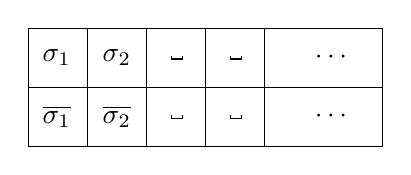
\begin{tikzpicture}
          \draw (5.25, 0.75) -- (9.75, 0.75);
          \draw (5.25, 0) -- (9.75, 0);
          \draw (5.25, 0) -- (5.25, 0.75);
          \draw (9.75, 0) -- (9.75, 0.75);

          \draw (5.25, 0) -- (5.25, 0.75);
          \draw (6, 0) -- (6, 0.75);
          \draw (6.75, 0) -- (6.75, 0.75);
          \draw (7.5, 0) -- (7.5, 0.75);
          \draw (8.25, 0) -- (8.25, 0.75);

          \node at (9.125, 0.375) {$\cdots$};
          \node at (7.125, 0.375) {\blank};
          \node at (7.875, 0.375) {\blank};
          \node at (5.6125, 0.375) {$\sigma_1$};
          \node at (6.375, 0.375) {$\sigma_2$};


          \draw (5.25, -0.75) -- (9.75, -0.75);
          \draw (5.25, -0.75) -- (5.25, 0);
          \draw (9.75, -0.75) -- (9.75, 0);

          \draw (5.25, 0) -- (5.25, -0.75);
          \draw (6, 0) -- (6, -0.75);
          \draw (6.75, 0) -- (6.75, -0.75);
          \draw (7.5, 0) -- (7.5, -0.75);
          \draw (8.25, 0) -- (8.25, -0.75);

          \node at (9.125, -0.375) {$\cdots$};
          \node at (7.125, -0.375) {\blank};
          \node at (7.875, -0.375) {\blank};
          \node at (5.6125, -0.375) {$\polneut{\sigma_1}$};
          \node at (6.375, -0.375) {$\polneut{\sigma_2}$};
        \end{tikzpicture}
      \end{center}
    \end{minipage}
    \begin{minipage}{0.38\textwidth}
      \trewwin{\sigma_1}{\sigma_2}{\blank}{\polneut{\sigma_1}}{\polneut{\sigma_2}}{\blank}
    \end{minipage}
  \end{overlayarea}

  \vspace{2ex}
  \onslide<2->
  \begin{center}

    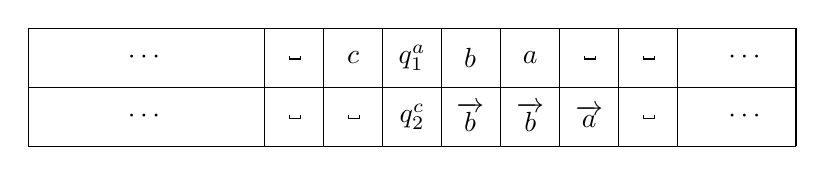
\begin{tikzpicture}
      \draw (0, 0.75) -- (9.75, 0.75);
      \draw (0, 0) -- (9.75, 0);
      \draw (0, 0) -- (0, 0.75);
      \draw (9.75, 0) -- (9.75, 0.75);

      \draw (4.5, 0) -- (4.5, 0.75);
      \draw (5.25, 0) -- (5.25, 0.75);
      \draw (3.75, 0) -- (3.75, 0.75);
      \draw (3, 0) -- (3, 0.75);
      \draw (6, 0) -- (6, 0.75);
      \draw (6.75, 0) -- (6.75, 0.75);
      \draw (7.5, 0) -- (7.5, 0.75);
      \draw (8.25, 0) -- (8.25, 0.75);

      %\node at (5.6125, 1) {\small$1$};
      %\node at (6.375, 1) {\small$2$};
      %\node at (7.125, 1) {\small$3$};
      %\node at (4.875, 1) {\small$0$};
      %\node at (4.125, 1) {\small$-1$};
      %\node at (3.375, 1) {\small$-2$};

      \node at (1.5, 0.375) {$\cdots$};
      \node at (9.125, 0.375) {$\cdots$};
      \node at (5.6125, 0.375) {$b$};
      \node at (6.375, 0.375) {$a$};
      \node at (7.125, 0.375) {\blank};
      \node at (7.875, 0.375) {\blank};
      \node at (4.875, 0.375) {$q_1^a$};
      \node at (4.125, 0.375) {$c$};
      \node at (3.375, 0.375) {\blank};

      %\path[<->] (0, 1.5) edge node[fill=white, anchor=center, pos= 0.5] {\small $z$} (4.5, 1.5);
      %\node[color=white] at (4.75, 1.5) {l};
      %\path[<->] (5.25, 1.5) edge node[fill=white, anchor=center, pos =0.5] {\small $z$} (9.75, 1.5);

      \draw (0, -0.75) -- (9.75, -0.75);
      \draw (0, -0.75) -- (0, 0);
      \draw (9.75, -0.75) -- (9.75, 0);

      \draw (4.5, 0) -- (4.5, -0.75);
      \draw (5.25, 0) -- (5.25, -0.75);
      \draw (3.75, 0) -- (3.75, -0.75);
      \draw (3, 0) -- (3, -0.75);
      \draw (6, 0) -- (6, -0.75);
      \draw (6.75, 0) -- (6.75, -0.75);
      \draw (7.5, 0) -- (7.5, -0.75);
      \draw (8.25, 0) -- (8.25, -0.75);

      \node at (1.5, -0.375) {$\cdots$};
      \node at (9.125, -0.375) {$\cdots$};
      \node at (5.6125, -0.375) {$\polpos{b}$};
      \node at (6.375, -0.375) {$\polpos{b}$};
      \node at (7.125, -0.375) {$\polpos{a}$};
      \node at (7.875, -0.375) {\blank};
      \node at (4.875, -0.375) {$q_2^c$};
      \node at (4.125, -0.375) {\blank};
      \node at (3.375, -0.375) {\blank};
    \end{tikzpicture}
  \end{center}
\end{frame}

\begin{frame}{Tableau}
  \begin{center}
    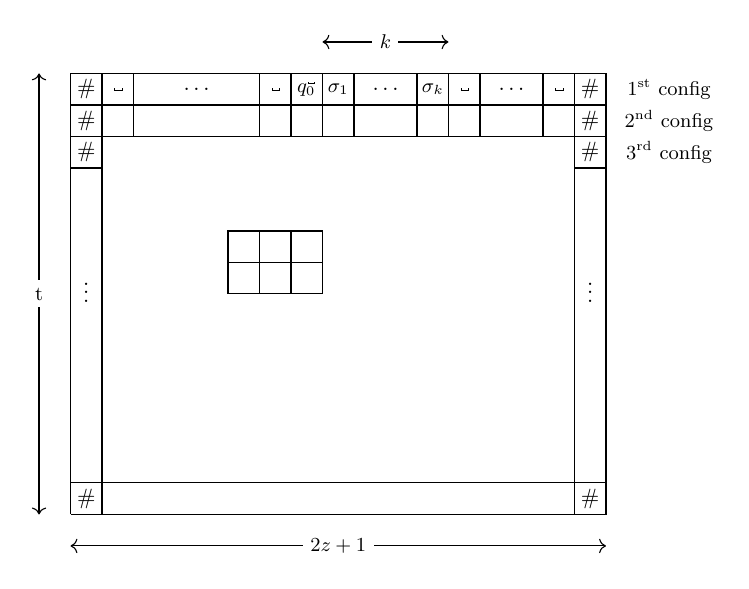
\begin{tikzpicture}[scale=0.8, every node/.style={scale=0.8}]
      \draw (1.5, -4) -- (1.5, 3) -- (10, 3) -- (10, -4) -- (1.5, -4);
      \draw (2, -4) -- (2, 3);
      \draw (2.5, 3) -- (2.5, 2);
      \draw (9.5, -4) -- (9.5, 3);
      \draw (1.5, 2.5) -- (10, 2.5);
      \draw (1.5, -3.5) -- (10, -3.5);
      \draw (1.5, 2) -- (10, 2);
      \draw (1.5, 1.5) -- (2, 1.5);
      \draw (9.5, 1.5) -- (10, 1.5);

      \draw (4.5, 3) -- (4.5, 2);
      \draw (5, 3) -- (5, 2);
      \draw (5.5, 3) -- (5.5, 2);
      \draw (6, 3) -- (6, 2);
      \draw (7, 3) -- (7, 2);
      \draw (7.5, 3) -- (7.5, 2);
      \draw (8, 3) -- (8, 2);
      \draw (9, 3) -- (9, 2);
      %\draw (2.5, 3) -- (2.5, 2);
      %\draw (3, 3) -- (3, 2.5);
      %\draw (4.5, 3) -- (4.5, 2.5);
      %\draw (5, 3) -- (5, 2.5);
      %\draw (5.5, 3) -- (5.5, 2.5);
      %\draw (7.5, 3) -- (7.5, 2.5);

      \node at (1.75, 2.75) {\#};
      \node at (1.75, 2.25) {\#};
      \node at (1.75, 1.75) {\#};
      \node at (1.75, -3.75) {\#};
      \node at (9.75, 2.75) {\#};
      \node at (9.75, 2.25) {\#};
      \node at (9.75, 1.75) {\#};
      \node at (9.75, -3.75) {\#};

      \node at (2.25, 2.75) {\textvisiblespace};
      \node at (3.5, 2.75) {$\ldots$};
      \node at (4.75, 2.75) {\textvisiblespace};
      \node at (5.25, 2.75) {\small $q_0^{\blank}$};
      \node at (5.75, 2.75) {\small $\sigma_1$};
      \node at (6.5, 2.75) {$\ldots$};
      \node at (7.25, 2.75) {\small $\sigma_k$};
      \node at (7.75, 2.75) {\textvisiblespace};
      \node at (8.5, 2.75) {$\ldots$};
      \node at (9.25, 2.75) {\textvisiblespace};

      %\node at (6.5, 2.75) {$\ldots$};
      %\node at (5, 2.25) {$\ldots$};

      \node at (1.75, -0.375) {$\vdots$};
      \node at (9.75, -0.375) {$\vdots$};

      \draw (4, -0.5) -- (4, 0.5) -- (5.5, 0.5) -- (5.5, -0.5) -- (4, -0.5);
      \draw (4.5, -0.5) -- (4.5, 0.5);
      \draw (5, -0.5) -- (5, 0.5);
      \draw (4, 0) -- (5.5, 0);

      \path[<->] (1, -4) edge node[fill=white, anchor=center, pos= 0.5] {\small t} (1, 3);
      \path[<->] (1.5, -4.5) edge node[fill=white, anchor=center, pos=0.5] {\small $2z + 1$} (10, -4.5);
      \path[<->] (5.5, 3.5) edge node[fill=white, anchor=center, pos=0.5] {\small $k$} (7.5, 3.5);

      \node at (11, 2.75) {\small 1\textsuperscript{st} config};
      \node at (11, 2.25) {\small 2\textsuperscript{nd} config};
      \node at (11, 1.75) {\small 3\textsuperscript{rd} config};
    \end{tikzpicture}
  \end{center} 
\end{frame}

\begin{frame}{Parallel Rewriting (\PR{})}
  Given: 
  \begin{itemize}
    \item an alphabet $\Sigma$ and a string length $l$
    \item an initial string $x_0 \in \Sigma^l$ and a step count $t$
    \item a width $w$ of rewrite windows 
      %and a rewriting offset $o$
    \item a set of rewrite windows $R$
    \item a set of final substring constraints $R_{\mathit{final}}$
  \end{itemize}
  Determine if there exists a sequence of strings $x_1, \ldots, x_t \in \Sigma^l$ s.t.\ 
  \begin{itemize}
    \item for every $0 \le i < t$ the rewrite is valid for $R$, denoted $x_i \rightsquigarrow x_{i+1}$: ``for all offsets, there exists a rewrite window''
    \item there exists an element $x \in R_{\mathit{final}}$ which is a substring of $x_t$
  \end{itemize}
\end{frame}

\begin{frame}{Nondeterminism}
  ``Guess'' an input string of length $\le k$ with a single rewrite step

  \vspace{2ex}
  Initial string: 
  \begin{center}
    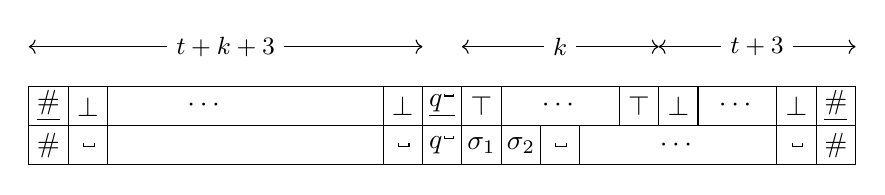
\begin{tikzpicture}
      \draw (0, 0.5) -- (10.5, 0.5);
      \draw (0, 0) -- (10.5, 0);
      \draw (0, 0) -- (0, 0.5);
      \draw (10.5, 0) -- (10.5, 0.5);

      \draw (0.5, 0.5) -- (0.5, 0);
      \draw (1, 0.5) -- (1, 0);
      \draw (10, 0.5) -- (10, 0);
      \draw (9.5, 0.5) -- (9.5, 0);
      \draw (5, 0.5) -- (5, 0);
      \draw (5.5, 0.5) -- (5.5, 0);
      \draw (4.5, 0.5) -- (4.5, 0);
      \draw (6, 0.5) -- (6, 0);
      \draw (7.5, 0.5) -- (7.5, 0);
      \draw (8, 0.5) -- (8, 0);
      \draw (8.5, 0.5) -- (8.5, 0);

      \node at (9, 0.25) {$\cdots$};
      \node at (6.75, 0.25) {$\cdots$};
      \node at (2.25, 0.25) {$\cdots$};

      \node at (0.25, 0.25) {\underline{\#}};
      \node at (0.75, 0.24) {$\bot$};
      \node at (4.75, 0.25) {$\bot$};
      \node at (5.25, 0.25) {$\underline{q^{\blank}}$};
      \node at (5.75, 0.25) {$\top$};
      \node at (7.75, 0.25) {$\top$};
      \node at (8.25, 0.25) {$\bot$};
      \node at (9.75, 0.25) {$\bot$};
      \node at (10.25, 0.25) {\underline{\#}};

      \onslide<2-> {
        \draw (0, -0.5) -- (10.5, -0.5);
        \draw (0, 0) -- (0, -0.5);
        \draw (10.5, 0) -- (10.5, -0.5);

        \draw (0.5, -0.5) -- (0.5, 0);
        \draw (1, -0.5) -- (1, 0);
        \draw (10, -0.5) -- (10, 0);
        \draw (9.5, -0.5) -- (9.5, 0);
        \draw (5, -0.5) -- (5, 0);
        \draw (5.5, -0.5) -- (5.5, 0);
        \draw (4.5, -0.5) -- (4.5, 0);
        \draw (6, -0.5) -- (6, 0);
        \draw (6.5, -0.5) -- (6.5, 0);
        \draw (7, -0.5) -- (7, 0);
        %\draw (7.5, -0.5) -- (7.5, 0);
        %\draw (8, -0.5) -- (8, 0);
        %\draw (8.5, -0.5) -- (8.5, 0);

        \node at (0.25, -0.25) {\#};
        \node at (0.75, -0.25) {\blank};
        \node at (4.75, -0.25) {\blank};
        \node at (5.25, -0.25) {$q^{\blank}$};
        \node at (5.75, -0.25) {$\sigma_1$};
        \node at (6.25, -0.25) {$\sigma_2$};
        \node at (6.75, -0.25) {\blank};
        \node at (8.25, -0.25) {$\cdots$};
        \node at (9.75, -0.25) {\blank};
        \node at (10.25, -0.25) {\#};
      }

      \path[<->] (5.5, 1) edge node[fill=white, anchor=center, pos= 0.5] {\small $k$} (8, 1);
      \path[<->] (0, 1) edge node [fill = white, anchor=center, pos=0.5] {\small $t + k + 3$} (5, 1);
      \path[<->] (8, 1) edge node [fill = white, anchor =center, pos=0.5] {\small $t + 3$} (10.5, 1);
    \end{tikzpicture}
  \end{center}
\end{frame}

\section{Formalisation}

\begin{frame}{Representation Relations}
  Representation of half-tapes $u \reprtt{p}{n} h$:
  \begin{itemize}
    \item $\length{u} \le n$
    \item $h = \textsf{mapPolarity}~p~u \con E_{\hat{n} - \length{u}}$
  \end{itemize}
  where $\hat{n} = n + 2$ and $E_n := \blank^n \#$. 
  \vspace{2ex}

  Representation of configurations $(q, \mathit{tape}) \reprc{} (ls, qm, rs)$: 
  \begin{itemize}
    \item $\textsf{left}~\mathit{tape} \reprtt{p}{z} ls$
    \item $qm = q^{\textsf{current}~\mathit{tape}}$
    \item $\textsf{right}~\mathit{tape} \reprtt{p}{z} rs$
  \end{itemize}

  \begin{align*}
    (q, \mathit{tp}) \reprc{} s := \exists ls~qm~rs,& s = \rev{(ls)} \con [qm] \con rs \\
    \land &(q, \mathit{tp}) \reprc{} (ls, qm, rs)
  \end{align*}
\end{frame}


\begin{frame}{Deterministic Simulation}
  \begin{center}
  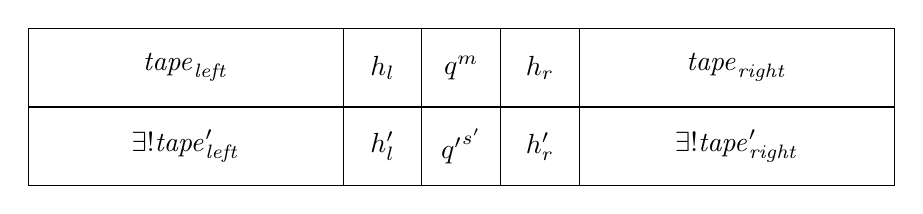
\begin{tikzpicture}
    \draw (0, 0) -- (11, 0);
    \draw (0, 1) -- (11, 1);
    \draw (0, 0) -- (0, 1);
    \draw (11, 0) -- (11, 1);

    \draw (4, 0) -- (4, 1);
    \draw (5, 0) -- (5, 1);
    \draw (6, 0) -- (6, 1);
    \draw (7, 0) -- (7, 1);

    \node at (2, 0.5) {$\mathit{tape}_{\mathit{left}}$};
    \node at (9, 0.5) {$\mathit{tape}_{\mathit{right}}$};
    \node at (4.5, 0.5) {$h_l$};
    \node at (6.5, 0.5) {$h_r$};
    \node at (5.5, 0.5) {$q^m$};

    \onslide<2-> {
      \draw (4, -1) -- (7, -1);
      \draw (4, -1) -- (4, 0);
      \draw (5, -1) -- (5, 0);
      \draw (6, -1) -- (6, 0);
      \draw (7, -1) -- (7, 0);

      \node at (4.5, -0.5) {$h_l'$};
      \node at (6.5, -0.5) {$h_r'$};
      \node at (5.5, -0.5) {${q'}^{s'}$};
    }

    \onslide<3-> {
      \draw (0, -1) -- (0, 0);
      \draw (11, -1) -- (11, 0);
      \draw (0, -1) -- (4, -1);
      \draw (7, -1) -- (11, -1);

      \node at (2, -0.5) {$\exists! \mathit{tape}_{\mathit{left}}'$};
      \node at (9, -0.5) {$\exists! \mathit{tape}_{\mathit{right}}'$};
    }

  \end{tikzpicture}
\end{center}
  %Somehow portray the idea that everything (flow of information) is propagated from the center of the string; the rewrite is determined uniquely by the head.

  %Then: rewrites for tape halves can be proven separately using only a subset of the rules
\end{frame}

\begin{frame}{Challenges}
  \begin{itemize}
    \item massive number of cases (100): proof \emph{heavily} relies on automation

      $\rightarrow$ rewrite rules formalised as inductive predicates
    \item proofs that rewrites are unique require \emph{a lot} of inversions
    \item left half of the tape is reversed compared to the Turing machine formalisation

      $\rightarrow$ use symmetry of rewrite rules for tapes
    \item Turing machine formalisation does not have notion of blanks
  \end{itemize}
\end{frame}

\section{Context}
\begin{frame}{Reduction of \PR{} to \sat{}}
  \begin{center}
    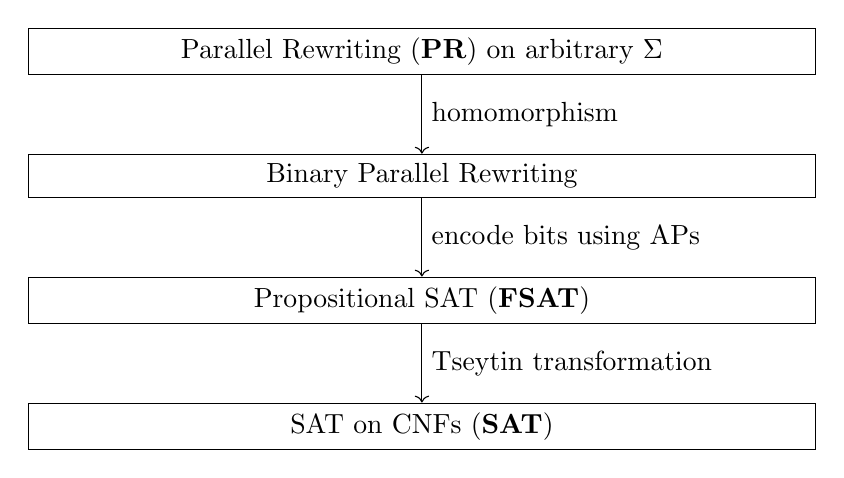
\begin{tikzpicture}
      \node[rectangle, draw=black, minimum width = 10cm] (strrew1) {Parallel Rewriting (\PR{}) on arbitrary $\Sigma$};
      \node[rectangle, draw=black, below = of strrew1, minimum width = 10cm] (strrew2) {Binary Parallel Rewriting};
      \node[rectangle, draw=black, below = of strrew2, minimum width = 10cm] (csat) {Propositional SAT (\fsat{})};
      \node[rectangle, draw=black, below = of csat, minimum width = 10cm] (sat) {SAT on CNFs (\sat{})};
      \draw[->] 
        (strrew1) edge node[right] {homomorphism} (strrew2)
        (strrew2) edge node[right] {encode bits using APs} (csat)
        (csat) edge node[right] {Tseytin transformation} (sat);
    \end{tikzpicture}
  \end{center}
\end{frame}

\begin{frame}{Conclusion}
  Contributions: 
  \begin{itemize}
    \item functional formalisation of Turing machine simulation in \PR{}
    \item heavy changes to the original proof\footnote{\cite{Sipser:TheoryofComputation}} to make inductive arguments work formally
  \end{itemize}

  \vspace{5ex}

  Roadmap:
  \begin{itemize}
    \item reduction of \PR{} to binary \PR{}
    \item reduction of binary \PR{} to formula satisfiablity
    \item (reduction of formula satisfiability to CNF satisfiability)
    \item extraction to L
  \end{itemize}
\end{frame}

\miniframesoff
\section{}

\begin{frame}{Transition Rules -- Examples}

\end{frame}

\begin{frame}{Tape Transformations}
  
\end{frame}

\begin{frame}{Step Simulation}
\end{frame}

\begin{frame}{Main Simulation Results}

\end{frame}

\begin{frame}{String Rewriting (SR) (and why it does not work for us)}
  \begin{itemize}
    \item rules $u/v$ where $u, v \in \Sigma^*$
    \item string rewriting system $R$ over $\Sigma$: finite set of rules
    \item rewrite relation $\Rightarrow_R$; given $x, y$, determine whether $x \Rightarrow_R^* y$ 
  \end{itemize}

  Problems: 
  \begin{itemize}
    \item only a single final string 
    \item essentially unbounded, would require a modified restricted version for \sat{}
    \item only a single rewrite in each step, does not allow tape shifting
  \end{itemize}
\end{frame}

\begin{frame}[allowframebreaks]{References}
  \nocite{Sipser:TheoryofComputation}
  \nocite{Bläser:TISkript}
  \bibliographystyle{apalike}
  \bibliography{references}{}
\end{frame}
\end{document}
